\label{parallel_sga}
Once applied successfully GA's are generally able to find good solutions to a problem in reasonable amounts of time. But when the problem in hand is bigger and harder, there is an increase in time required to find adequate solutions for it. Because of this there have been many efforts to make GA's faster by parallel implementation \citep{cantu:98}.

There are two possible ways of parallelising GA's. 
\begin{itemize}
	\item Data parallelism
	\item Task parallelism
\end{itemize}

\paragraph{Data parallelism}
Data parallelism is dividing up data in a program into multiple subsets and executing same procedure(s) on them. With data parallelism, parallelism grows with data.
\paragraph{Task parallelism}
Task parallelism involves concurrent execution of different operations on different processor in parallel on same data. Usually suitable for executing several procedures on same data where no dependencies between tasks.
\citep{konfrst:04para}

A hybrid parallelism by mixing both data and task parallelism is also common. Generally in GAs computation time increases with data therefore data parallelism is usually implemented for parallelising.

\subsection{Classification of Parallel GAs}
Many models of parallel GA implementation exist. These options are depend on answer to the questions such as how fitness are evaluated, how mutation and crossover operations are applied, if a single or multiple population are used, how individuals are exchanged, if selection applied globally or locally.

Luque et al \citep{luque:05} and Cant\'{u}-Paz\citep{cantu:98} classified parallel GA model into following categories:
\begin{itemize}
	\item {Master-slave model - Global population}
	\item {Distributed  model - Coarse grained}
	\item{Cellular model - Fine grained}
\end{itemize}

\subsection{Master-slave Model - Global population}
Similar to Simple GA, master-slave model consists a single global population. Usually the evaluation of fitness function is distributed among multiple processors. The main loop of the GA is executed in a master process. In this model of parallel GA selection and crossover consider the entire global population. One distinctive advantage of masters-slave model of parallel GA is that it does not alter the behaviour of the algorithm other than speeding up. This model is efficient as the objective function evaluation becomes more expensive to compute. Figure \ref{fig:pga_master_slave} shows the Master-slave model's message exchange between master and slave processes where slave process evaluate a part of the global population fitness value.

\begin{figure}[!htb]
\begin{center}
  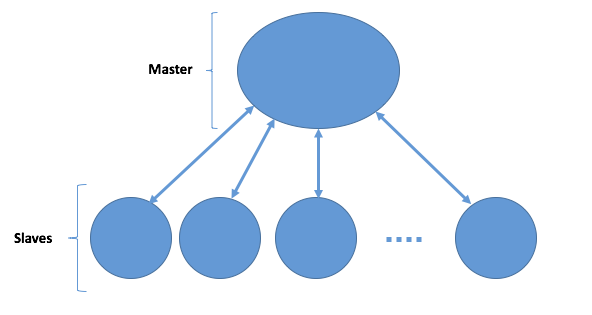
\includegraphics[width= 0.7 \linewidth]{figs/pga_master_slave.png}
  \caption{Master-Slave PGA model.}
  \label{fig:pga_master_slave}
  \end{center}
\end{figure}

\subsection {Distributed Model - Coarse grained}
In distributed model initial population are divided into relatively isolated subpopulations. These sub-population are called \textbf{\emph{island}}. This is also known as multi-population or multi-demes GAs. These islands evolve independently over time but allows individuals to be migrated to another island. The genetic operations selection, mutation and crossover are performed within the subpopulation of each island. Figure \ref{fig:pga_distributed} shows the distributed model of PGA where each node independently performs all GA operation on it's local population for a generation and then the best individual is migrated to the next neighbour.

\begin{figure}[!htb]
\begin{center}
  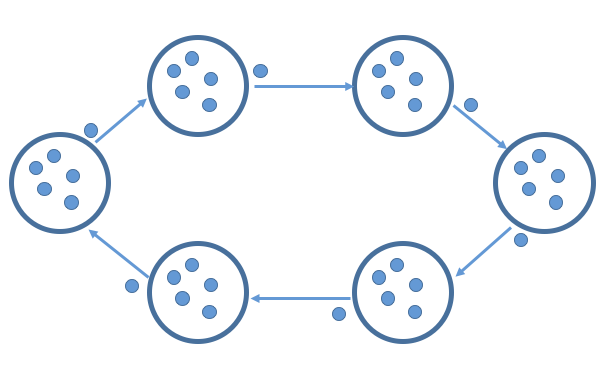
\includegraphics[width= 0.7 \linewidth]{figs/pga_distributed.png}
  \caption{Distributed PGA model.}
  \label{fig:pga_distributed}
  \end{center}
\end{figure}

\subsection{Cellular Model - Fine grained}
Cellular or fine-grained parallel GAs works on one single population where each processing unit holds only one or two individuals hence its called fine-grained. This model structures the global population into neighbourhoods where individuals can only interact with their neighbours only. Which limits an individual only to compete and mate with its neighbouring individuals. Therefore a good solution can arise in different area of the population distribution and can spread throughout the whole population overtime. Cellular GAs are originally designed for massively parallel machines. Figure \ref{fig:pga_cellular} shows the cellular PGA model where each node holds one or two individuals and interact with all immediate neighbours for selecting other individuals to perform local GA operation to reproduce offsprings. 

\begin{figure}[!htb]
\begin{center}
  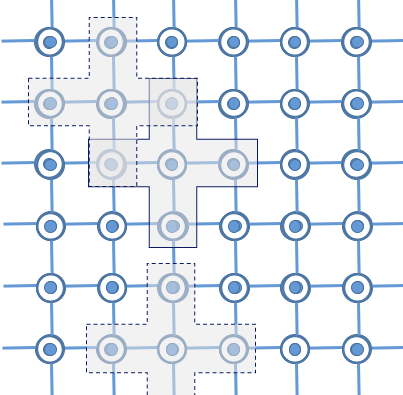
\includegraphics[width=.5 \linewidth]{figs/pga_cellular.png}
  \caption{Cellular PGA model.}
  \label{fig:pga_cellular}
  \end{center}
\end{figure}


